%# -*- coding: utf-8-unix -*-
%%==================================================
%% chapter02.tex for SJTU Master Thesis
%% based on CASthesis
%% modified by wei.jianwen@gmail.com
%% Encoding: UTF-8
%%==================================================

\chapter{相关工作与技术}
\label{chap:example}
本文研究的竞争感知的混合线程放置框架主要基于CSTMCS锁实现,而CSTMCS锁是适用于NUMA架构的两层的MCS锁。所以本章主要介绍NUMA架构,MCS锁,CSTMCS锁、线程调度/放置及与之相关的技术。

\section{NUMA架构及相关优化技术}
\begin{figure}[t]
	\centering
	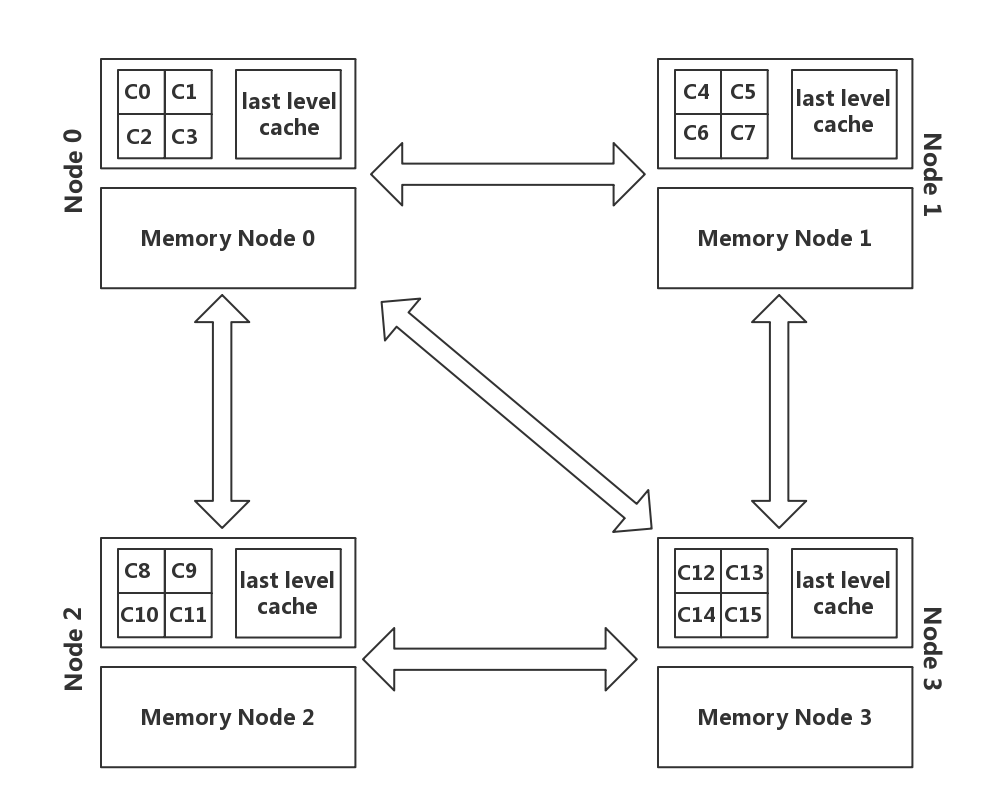
\includegraphics[width=5.0in]{NUMA.PNG}
	\caption{由四个四核处理器组成的NUMA系统}
	\label{Fig:numa}
\end{figure}
大型现代服务器通常有多个处理器节点组成,每个节点包含一个多核处理器和一块本地内存,其中本地内存上一般会有一个或多个内存控制器(memory controller)来处理来自本地节点或者其他节点上地核地内存访问请求,如图\ref{Fig:numa}所示。所有计算节点之间通过高速通信介质(interconnect)连接成单个缓存一致性系统,虽然物理内存被分割在了多个节点上,但是逻辑上物理地址空间仍然是全局共享的,也就是说所有核能够透明地访问所有节点上地物理内存。计算核心直接通过本地内存控制器来访问本地内存,而访问远程内存时则要通过节点间通信介质核远程内存地内存控制器。访问远程内存通常要比访问本地内存花费更多地时间,所以这些系统都具有非一致性内存访问时间(Non-Uniform Memory access, NUMA)地特征。再考虑到内存和缓存地层级化(memory hierarchy)设计,这张访存地非一致性更加显著。

显然要使应用程序在NUMA架构上获得最佳的性能,在放置应用程序地线程和内存数据地时候必须考虑系统资源的物理构成和分布,比如为了充分利用访存操作的局部性,将线程及其访问的数据放置在同一个node上来避免远程内存访问的巨大开销。由于NUMAnu'm架构的服务器的广泛应用,目前很多操作系统都针对NUMA因素做了通用的优化,比如很多Linux系统都提供了numactl用于查看和优化NUMA系统中的线程放置和内存管理。使用numactl中的numastat用户可以查看各个NUMA节点的内存分配和节点之间的内存访问状况,比如查看每个节点上运行的进程在该节点和其他节点上各申请了多少内存。通过设置numactl的参数用户可以限定应用只能运行在某些NUMA特定NUMA节点集合或者核集合上或者限定该应用的内存只能分配在某些NUMA节点集合上。除此以外,numactl还可以设置更为复杂的内存分配核管理策略,比如是否使用巨页(huge page),内存是否交织(interleave)分布在所有或者某些节点上。

上述操作系统提供的的这些优化工具一方面时非常粗粒度的,另一方面要求用户必须实现了解所运行的程序的特征,而现实的应用特征时复杂多变的而且事先难以预测的,所以仅靠这些通用工具很难最大化应用的性能,进一步的优化必须监测和考虑应用程序本身的特征。Carrefour\cite{dashti2013traffic}在分析了大量应用程序的访存特征后,认为应该根据应用的内存访问特征来使用合适的内存放置和管理策略,如图\ref{Fig:carrefour}所示,Carrefour支持三种内存访问策略:
\begin{itemize}
\item  复制(replication),即将同一个页的拷贝放置在多个NUMA节点上,复制将热点数据的访问压力分摊到了多个内存控制器,同时避免了远程内存访问,但是必须保持多个复制页内容一致,类似于缓存一致性,代价非常高昂,所以一般只对读写比很高的页采用复制策略;
\item  交织(interleaving),即将内存页平均放置在所有节点上,从而平衡各个内存控制器和节点间通信介质的访问压力,操作系统提供的交织时全局性的,而Carrefour中的交织可以只对部分页使用,进行更细力度的内存管理;
\item 协同放置(co-locate),即将共享内存页的线程于其共享的内存页放置在同一个节点上,从而减少远程内存访问和缓存一致性操作。
\end{itemize}

\begin{figure}[t]
	\centering
	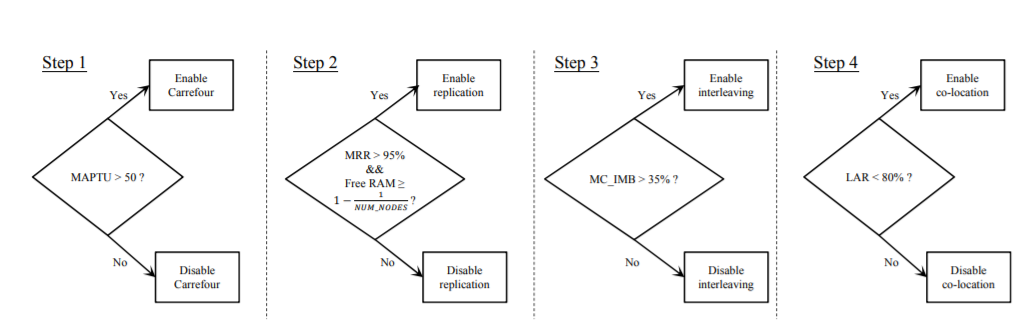
\includegraphics[width=5.6in]{Carrefour.PNG}
	\caption{Carrefour中的内存放置策略选择}
	\label{Fig:carrefour}
\end{figure}

\section{MCS锁与CSTMCS锁}
\subsection{MCS锁}
MCS锁是一种基于单项链表的高性能、可扩展、公平的自旋锁,由John Mellor-Crummey和Michael在1991年提出, Scott其名称来源于发明人的名字首字母。MCS锁具有以下四个特征:
\begin{itemize}
\item  保证FIFO(first-in, first-out)的拿锁顺序;
\item  每个线程只在本地标志变量上自旋;
\item  每个锁本身只占用很小的常数大小的内存空间;
\item  不管有没有缓存一致性,性能都很好;
\end{itemize}

如图\ref{Fig:MCS}的伪代码所示,MCS锁中包含一个指向对尾的指针tail,每个竞争者在队列中用一个记录(record)表示,其中每个记录包含一个指向后继节点的指针和一个表示当前是否拿到锁的布尔变量。每个线程需要拿锁时使用compare\_and\_swap这个原子操作来完成以下操作将自身的记录加入队列:1)使tail指针指向自己的记录;2)将自己的记录连接在前去节点(如果有的话)的后面。如果该线程有前驱节点,则它在自身记录的布尔变量上自旋直到拿到锁,否则直接进入关键区域。放锁时只需要将后记节点的记录中的布尔变量设为true即可,如果没有后继节点则将tail设为null。

MCS的FIFO的公平性是通过显式存在的队列来维持的,其正确性由算法本身和compare\_and\_swap这个原子操作共同保证,每个线程旨在本地标志变量上自旋并且只有自身还前驱节点对应的线程会访问该变量,这是MCS锁获得高性能和可扩展性的主要原因。
\begin{figure}[t]
	\centering
	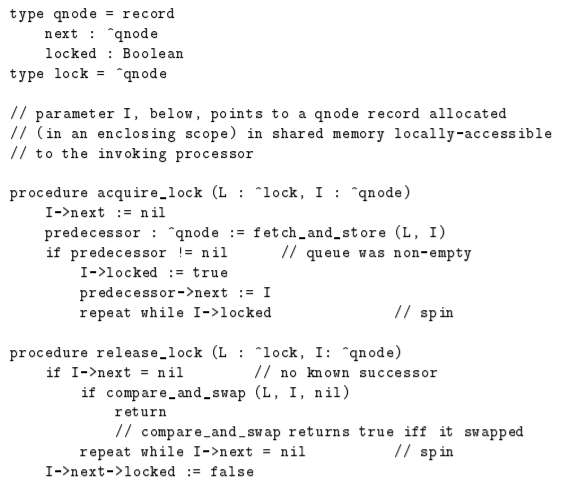
\includegraphics[width=5.6in]{MCS.PNG}
	\caption{基于队列的MCS锁}
	\label{Fig:MCS}
\end{figure}

\subsection{CSTMCS锁}
CSTMCS锁是针对NUMA架构下内存及缓存访问的非一致性而对MCS锁做的适应性改进。它是CST锁的基础部分,也可以看作是一个两层的cohort MCS锁。如图\ref{Fig:CSTMCS}所示,该示例中展示了一个有9个线程的多线程应用,每个线程都差不多在同一个时刻竞争同一个锁(具体顺序如图(a)所示),其中线程T1到T5在节点0上而另外四个线程在节点1上,图a表示使用MCS锁时按照FIFO的顺序会有6次跨NUMA节点的锁传递(黄色表示跨节点锁传递),图b表示如果对锁的传递顺序加以合理调度则可以将跨节点的锁传递次数将为1,从而改善MCS锁在NUMA架构下的性能。a,b两图展示了CSTMCS锁和MCS锁的本质差别,即CSTMCS通过改变MCS锁的锁调度顺序,牺牲一定的短期公平性来减少跨节点的锁传递频率,获得更好的性能。

CSTMCS的具体实现还是以MCS锁为基础,包含一个全局MCS锁和每个节点上的一个局部MCS锁。全局MCS锁在所有节点之间共享,它的主要作用时将竞争分隔在各个节点内;而每个局部MCS锁只在其锁在的节点内的线程间共享。一个线程只有同时拿到全局MCS锁和其所在节点的局部MCS锁才可以进入关键区域。锁的锁传递顺序可以描述为,锁的持有者将其传给一个本地的最早请求者当且仅当以下两个条件同时满足:
\begin{itemize}
\item  本地节点当前至少有一个请求者;
\item  所在本地节点的传递次数还未超过预先设定的threshold;
\end{itemize}
其中设置threshold是为了防止深层的不公平。

CSTMCS锁在决定锁的调度顺序时考虑了等待队列中的线程和当前拿锁线程在NUMA拓扑上的相对位置,从而让减少了锁在NUMA节点之间的迁移频率,提高锁的总吞吐率。相反的,标准的MCS锁不能感知底层的NUMA因素,所以只能按照线程的到达时间即线程请求锁的时间来决定锁的传递顺序,所以在NUMA架构上会有性能损失。当然,CSTMCS锁的高吞吐率是以牺牲一定的短期公平性为代价的。
\begin{figure}[t]
	\centering
	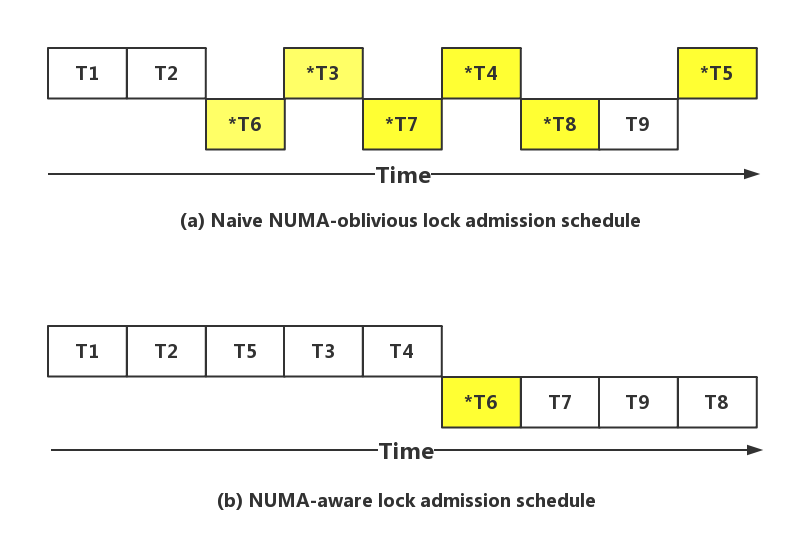
\includegraphics[width=5.6in]{CSTMCS.PNG}
	\caption{CSTMCS锁示例}
	\label{Fig:CSTMCS}
\end{figure}

\section{线程调度与放置}
\subsection{Linux线程调度}
作为资源管理的核心部分,操作系统的线程调度器的主要职责是保证准备好的线程被调度到可用的核上去。在Linux系统当前使用的调度算法CFS(Completely Fair Scheduling)\cite{lozi2016linux}是WFQ(Weighted Fair Queueing)调度算法的一种实现。在单CPU系统中,CFS的实现非常简单。为了实现公平调度,CFS定义了一个固定长度的时间间隔,在该间隔内系统中的每个线程至少运行一次,该间隔被按照线程的权重按比例分为若干个大小不一的时间片(time slice),每个线程的权重就是它的优先级。正在运行的线程会不断增加它的已运行时间(vruntime),当它的vruntime超过分配给其的时间片时,如果当前有其他可以运行的线程,那么正在运行的线程就会被抢占;另外当前运行的线程也可能被另一个被唤醒的vruntime更小的线程抢占。具体的实现中,线程被组织为一个用红黑树实现的运行队列(runqueue),在该运行队列中,每个线程按照其vruntime排序,当CPU需要找一个线程来运行的时候,红黑树中最左边的线程也就是vruntime最小的线程会被选择。

在NUMA架构下,由于缓存一致性和同步机制等的巨大代价及内存访问非一致性等原因的存在使得CFS的实现变得非常复杂。为了保持良好的可扩展性,CFS使用了per-core runqueue,即每个核一个运行队列,这样设计大的主要原因是进程切换(context switch)发生在关键路径上而每个核一个运行队列使得进程切换时只需要访问本地运行队列。这与但是为了使调度算法在使用了per-core runqueue时能够正确高效的运行,必须有额外的机制来保持运行队列的负载均衡。Linux CFS采用的方法是周期性地运行一个负载均衡算法来保持所有队列负载地大致均衡,具体实现中采用了层级化地策略(hierarchy strategy),所有核被逻辑上组织为一个层次结构,该层次结构的最底部是单个核,这些核在下一层及后面个岑被如何分组是由它们对物理资源(内存,各级缓存)的共享拓扑决定的。每层的结构被称为一个调度域(scheduling domain),负载均衡算法按照自下而上的顺序在每个调度域内运行。将所有核组织成一个层次结构然后自下而上运行负载均衡算法相比直接在所有核之间通过线程迁移来调节负载的主要优势在于可以减少跨深层NUMA因素的线程迁移比例从而使得负载均衡算法的开销尽可能地小,这与层级锁的设计思路很相似。

现代操作系统的调度器在做线程调度时主要考虑因素有三点:1)通过线程在核之间的迁移来保证可运行的线程能被调度到可用的核上去;2)保证核之间负载的大致均衡;3)在NUMA架构下使负载均衡算法的代价尽可能大地小。这种调度算法非常适合相互之间没有关系地线程即不通过共享内存通信地线程,它能够避免线程之间对于节点层次地共享资源例如缓存、内存通道等地使用发生冲突(缓存失效等),它的前提假设是线程之间地通信非常少并且远不如节点层次地本地资源使用冲突重要。但是在锁集中并且存在大量线程间共享数据的多线程应用中,显然线程之间的通信是居于主导地位的,保证线程之间通信的高效的重要性显然要高过线程对资源的独享重要性\cite{dice2015lock},所以操作系统通用的调度器显然不能很好的满足这类场景的需求。另外考虑到层级锁中通过挖掘线程之间的亲和性来做锁调度,而通用的调度器将相关的线程分散在所有节点的可用核上使得层级锁可以挖掘的线程间的亲和性非常有限。

综上来看,通用的调度器并不适合NUMA架构下锁集中的多线程应用尤其是使用层级锁多线程的应用,为了使这些应用获得更好的性能,必须有定制化的考虑应用具体特征的线程调度/放置方法,也就是说应该使用定制化的调度器或者让应用程序来做自身的线程调度/放置。


\subsection{NUMA架构下的线程放置/迁移}

\begin{figure}[t]
	\centering
	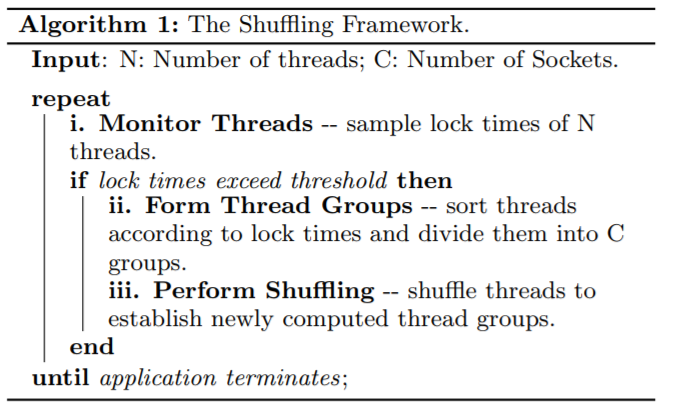
\includegraphics[width=5.6in]{shuffling.PNG}
	\caption{shuffling 框架}
	\label{Fig:shuffling}
\end{figure}
在NUMA架构下,操作系统的通用调度器很容易造成锁在NUMA节点之间的频繁迁移进而导致其性能下降,所以出现了很多定制化的线程放置/迁移策略,比如最朴素的做法是将请求锁的线程迁移到当前持锁的线程锁在的节点,即将线程迁移到包含锁及其保护的数据的缓存而不是相反,然而这张简单的迁移存在两个问题:1)线程迁迁移次数不可控;2)容易导致负载不均衡,最终的结果可能是得不偿失。shuffling\cite{pusukuri2014shuffling}是一种能够兼顾负载均衡核迁移代价的适合锁集中的应用的线程放置/迁移策略。shuffling通过将到达时间(lock arrival time)差不多的线程放置在相同的节点上来避免锁在节点间随意迁移,具体做法如图\ref{Fig:shuffling}所示,shuffling周期性地收集各个线程地到达时间;然后按照到达时间将所有线程排序分组,到达时间相似地线程被分到相同地组里,每组地大小等于每个节点上地计算核心数;最后通过迁移某些线程将分好地每个线程组映射到NUMA节点上去。相比简单地线程迁移,shuffling保证了负载均衡并且可以很好地控制线程地迁移。

在层级锁中,上述将请求锁线程迁移到当前持锁线程锁在NUMA节点上显然是没有必要的,因为层级锁并不是按原有锁的传递顺序来传递的。层级锁通过利用线程之间的亲和性来调度锁进而减少锁在节点间的迁移,所以对于层级锁来说最自然最高效的线程放置策略就是在保持负载均衡地前提下将线程尽可能地放地紧凑,所以大多数地层级锁将每个线程绑定到一个专用地核上,只有当前地节点上没有可用地核时才会将新的线程放置在一个新的节点上。此外,也有地层级锁出于测试锁地某些方面地表现等其他目的而将线程平均放置在所有节点上。我们在下一章中会对这两种线程放置策略进行进一步地分析和说明。

\section{本章小结}
本章主要对本文研究所基于地平台和技术进行了说明,包括NUMA架构地特性及相关的优化技术,MCS锁、CSTMCS锁的实现及特性,Linux系统下的通用调度器的特性及其局限性,还有针对锁集中的应用的一些线程放置策略及其优化等。这些相关的研究和技术一方面时本文研究的基石,另一方面也为本文的研究提供了很多有益的启发和借鉴,比如本文的提出的线程放置框架的混合特性与Carrefour的混合内存放置策略相似,为了保证长期公平性而使用的shift机制与Malthusian锁的shift机制的做法和目的都很相似,而竞争感知的特性则是借鉴了AHMCS锁的竞争感知。